%\documentclass[notitlepage,aps,prd,twocolumn,nofootinbib]{revtex4-1}
\documentclass[notitlepage,aps,prd,nofootinbib]{revtex4-1}

\usepackage{subfig}
%\usepackage[colorinlistoftodos]{todonotes}
\usepackage{float}

%\usepackage[protrusion=true,expansion=true]{microtype}
\usepackage{amsmath}
\usepackage{amssymb}
\usepackage{bbm}
\usepackage{ulem}
%\usepackage{feynmp-auto}
%\usepackage{slashed}
%\usepackage[absolute,overlay]{textpos}
\usepackage[usenames, dvipsnames]{color}
\usepackage{graphicx}
\usepackage{listings}
\usepackage{epsfig}
\usepackage{hyperref}
%\usepackage{tikz}
\usepackage{enumerate}
%\usepackage{fixltx2e} % buggy
\usepackage[compatibility=false]{caption}
%\usepackage{subcaption} % doesn't work with subfigure
\usepackage{pdfpages}
%\usepackage{setspace}
\usepackage{verbatim}

\DeclareRobustCommand{\orderof}{\ensuremath{\mathcal{O}}}

\definecolor{dukeblue}{RGB}{0,0,156}
\definecolor{dukedarkblue}{RGB}{0,26,87}
\definecolor{dukeblack}{RGB}{79,79,79}
\definecolor{dukegray}{RGB}{79,79,79}
\definecolor{dukesecbrown}{RGB}{217,200,158}
\definecolor{dukesecblue}{RGB}{127,169,174}

%\renewcommand*{\thefootnote}{\fnsymbol{footnote}}

%%%%%%%%%%%%%%%%%%%%%%%%%%%%%%%%%%%%%%%%%%%%%%%%%%%%%%%%%%%%%%%%%%%%%%%%%%%%%%%%%%%%%
\hypersetup{
    breaklinks,
    baseurl       = http://,
    pdfborder     = 0 0 0,
    pdfpagemode   = UseNone,% do not show thumbnails or bookmarks on opening
    pdfstartpage  = 1,
    bookmarksopen = true,
    bookmarksdepth= 2,% to show sections and subsections
% revtex needs author and title declared after \begin{document}, so have to hard code them...
%    pdfauthor     = {\@author},
%    pdftitle      = {\@title},
    pdfauthor     = {Matthew Epland},
    pdftitle      = {Phys 566 HW2},
    pdfsubject    = {},
    pdfkeywords   = {}}


% Code import settings
%%%%%%%%%%%%%%%%%%%%%%%%%%%%%%%%%%%%%%%%%%%%%%%%%%%%%%%%%%%%%%%%%%%%%%%%%%%%%%%%%%%%%
\definecolor{mygreen}{rgb}{0,0.6,0}
\definecolor{mygray}{rgb}{0.5,0.5,0.5}
\definecolor{mymauve}{rgb}{0.58,0,0.82}

%\lstset{ %
\lstdefinestyle{python}{ %
  backgroundcolor=\color{white},   % choose the background color; you must add \usepackage{color} or \usepackage{xcolor}
  basicstyle=\scriptsize,          % the size of the fonts that are used for the code
  breakatwhitespace=false,         % sets if automatic breaks should only happen at whitespace
  breaklines=true,                 % sets automatic line breaking
  captionpos=b,                    % sets the caption-position to bottom
  commentstyle=\color{mygreen},    % comment style
  deletekeywords={...},            % if you want to delete keywords from the given language
  escapeinside={\%*}{*)},          % if you want to add LaTeX within your code
  extendedchars=true,              % lets you use non-ASCII characters; for 8-bits encodings only, does not work with UTF-8
  frame=single,	                   % adds a frame around the code
  keepspaces=true,                 % keeps spaces in text, useful for keeping indentation of code (possibly needs columns=flexible)
  keywordstyle=\color{blue},       % keyword style
  language=Python,                 % the language of the code
  otherkeywords={*,...},           % if you want to add more keywords to the set
  numbers=left,                    % where to put the line-numbers; possible values are (none, left, right)
  numbersep=5pt,                   % how far the line-numbers are from the code
  numberstyle=\tiny\color{mygray}, % the style that is used for the line-numbers
  rulecolor=\color{black},         % if not set, the frame-color may be changed on line-breaks within not-black text (e.g. comments (green here))
  showspaces=false,                % show spaces everywhere adding particular underscores; it overrides 'showstringspaces'
  showstringspaces=false,          % underline spaces within strings only
  showtabs=false,                  % show tabs within strings adding particular underscores
  stepnumber=5,                    % the step between two line-numbers. If it's 1, each line will be numbered
  stringstyle=\color{mymauve},     % string literal style
  tabsize=2,	                   % sets default tabsize to 2 spaces
%  title=\lstname                   % show the filename of files included with \lstinputlisting; also try caption instead of title
  title={\protect\filename@parse{\lstname}\protect\filename@base.\filename@ext},
  firstnumber=0,
%  linewidth=0.95\textwidth
  xleftmargin=0.01\textwidth,
  xrightmargin=0.01\textwidth
}

\lstdefinestyle{output}{ %
  backgroundcolor=\color{white},   % choose the background color; you must add \usepackage{color} or \usepackage{xcolor}
  basicstyle=\scriptsize,          % the size of the fonts that are used for the code
  breakatwhitespace=false,         % sets if automatic breaks should only happen at whitespace
  breaklines=true,                 % sets automatic line breaking
  captionpos=b,                    % sets the caption-position to bottom
  escapeinside={\%*}{*)},          % if you want to add LaTeX within your code
  frame=single,	                   % adds a frame around the code
  keepspaces=true,                 % keeps spaces in text, useful for keeping indentation of code (possibly needs columns=flexible)
  numbers=left,                    % where to put the line-numbers; possible values are (none, left, right)
  numbersep=5pt,                   % how far the line-numbers are from the code
  numberstyle=\tiny\color{mygray}, % the style that is used for the line-numbers
  rulecolor=\color{black},         % if not set, the frame-color may be changed on line-breaks within not-black text (e.g. comments (green here))
  stepnumber=5,                    % the step between two line-numbers. If it's 1, each line will be numbered
  tabsize=2,	                   % sets default tabsize to 2 spaces
%  title=\lstname                   % show the filename of files included with \lstinputlisting; also try caption instead of title
  title={\protect\filename@parse{\lstname}\protect\filename@base.\filename@ext},
  firstnumber=0,
%  linewidth=0.95\textwidth
  xleftmargin=0.01\textwidth,
  xrightmargin=0.01\textwidth
}


%%%%%%%%%%%%%%%%%%%%%%%%%%%%%%%%%%%%%%%%%%%%%%%%%%%%%%%%%%%%%%%%%%%%%%%%%%%%%%%%%%%%%
\begin{document}

\title{PHYS 566 HW2}
\author{Matthew Epland}
\affiliation{Department of Physics, Duke University, Durham, NC 27707, USA}
%\institute{Duke University}

\date{\today}

\begin{abstract}
Nuclear decay activity $R\left(t\right)$ was simulated numerically using the Euler method in the context of Carbon-14 dating. Three time steps of $\Delta t =$ 10, 100, and 100 years were used to model $R\left(t\right)$ over $20,000$ years. The numerical results were compared to the analytical solution and found to be consistent with \le1\% divergence after two half-lives for $\Delta t =$ 10 and 100 years, and inconsistent with 9.2\% divergence for $\Delta t =$ 100 years. For all three time steps the divergence observed was orders of magnitude smaller than the second order term of the analytical solution.
\end{abstract}\maketitle


\section{Introduction}
\label{sec:intro}
Carbon dating is an extremely useful tool for establishing the age of ancient objects in archeology and related fields. From a physics stand point the method is fairly simple, being an application of well understood nuclear decays. In this assignment we numerically modeled the decay of a $10^{-12}$ kg sample of Carbon-14, which has a half-life of 5700 years, over a period of 20,000 years in order to gain practice applying the Euler method to solve differential equations. Carbon dating is a good case study for doing so as the exact result, a decaying exponential, can by derived analytically without much issue.

\section{Theory}
\label{sec:theory}

The decay of atomic nuclei can be modeled by assuming the change in number of nuclei per unit time, $\frac{d N}{d t}$, is proportional to the number of nuclei present at the time, $N\left(t\right)$.

\begin{equation} \label{eq:deq}
\frac{d N}{d t} = -\frac{1}{\tau} N\left(t\right)
\end{equation}

This simple first-order differential equation (\ref{eq:deq}) can be solved using separation of variables, resulting in the familiar equation for exponential decay (\ref{eq:exp}).

\begin{equation} \label{eq:exp}
N\left(t\right) = N_{0} e^{-t/\tau}
\end{equation}

The exponential decay is characterized by initial number of nuclei present, $N_{0}$, and the decay constant, $\tau$. We can relate $\tau$ to the half-life of the nuclei, $T_{1/2}$, when half of the initial population has decayed by solving (\ref{eq:half-life}). Taking natural logs of both sides and rearranging gives the desired result, $T_{1/2} = \tau \ln\left(2\right)$.


\begin{equation} \label{eq:half-life}
\frac{N_{0}}{2} = N_{0} e^{-T_{1/2}/\tau}
\end{equation}

In this assignment we are interested in calculating the activity of the decay, $R\left(t\right)$, defined in (\ref{eq:activity}).

\begin{equation} \label{eq:activity}
R\left(t\right) \equiv -\frac{d N}{d t} = \frac{1}{\tau} N\left(t\right) = \frac{N_{0}}{\tau} e^{-t/\tau}
\end{equation}

To calculate $N\left(t\right)$, and hence $R\left(t\right)$, numerically we can use the Euler method; approximating the derivative over a finite time step $\Delta t$ as (\ref{eq:euler}).

\begin{equation} \label{eq:euler}
\frac{d N}{d t} \approx \frac{N\left(t+\Delta t\right)-N\left(t\right)}{\Delta t}
\end{equation}

Substituting (\ref{eq:deq}) in for $\frac{d N}{d t}$ in (\ref{eq:euler}) and solving for $N\left(t+\Delta t\right)$ produces an iterative equation (\ref{eq:N_approx}) which we can use to compute $N\left(t\right)$ and $R\left(t\right)$ in our program.

\begin{equation} \label{eq:N_approx}
N\left(t+\Delta t\right) = \tau R\left(t+\Delta t\right) = \left(1-\frac{\Delta t}{\tau}\right) N\left(t\right)
\end{equation}


\section{Results}
\label{sec:results}
As can be seen in Figures~\ref{fig:plot} and~\ref{fig:log_plot}, the Euler method numerical results using small time steps $\Delta t =$ 10, and 100 years are practically indistinguishable from the exact result when plotted. However, when $\Delta t$ is increased to 1000 years the numerical result begins to diverge visually.

\begin{figure}[!htbc]
%\begin{figure}
  \centering
  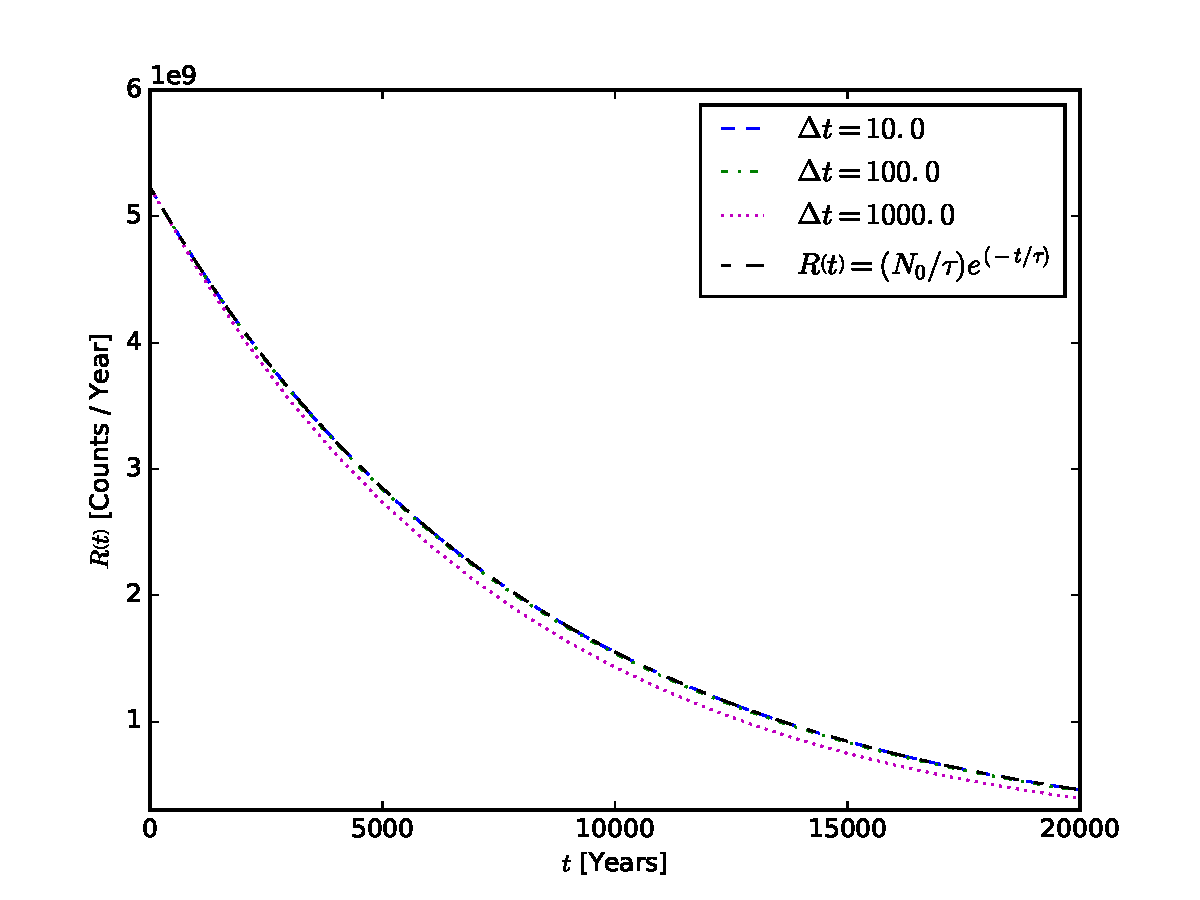
\includegraphics[width=.70\textwidth]{output/plot.pdf}
	{\par\nobreak\rule[9pt]{35em}{0.5pt}\vspace{-5mm}}
	\caption{$R\left(t\right)$ calculated numerically with three different time steps, $\Delta t$, and the exact solution.}
	\label{fig:plot}
\end{figure}

\begin{figure}[!htbc]
%\begin{figure}
  \centering
  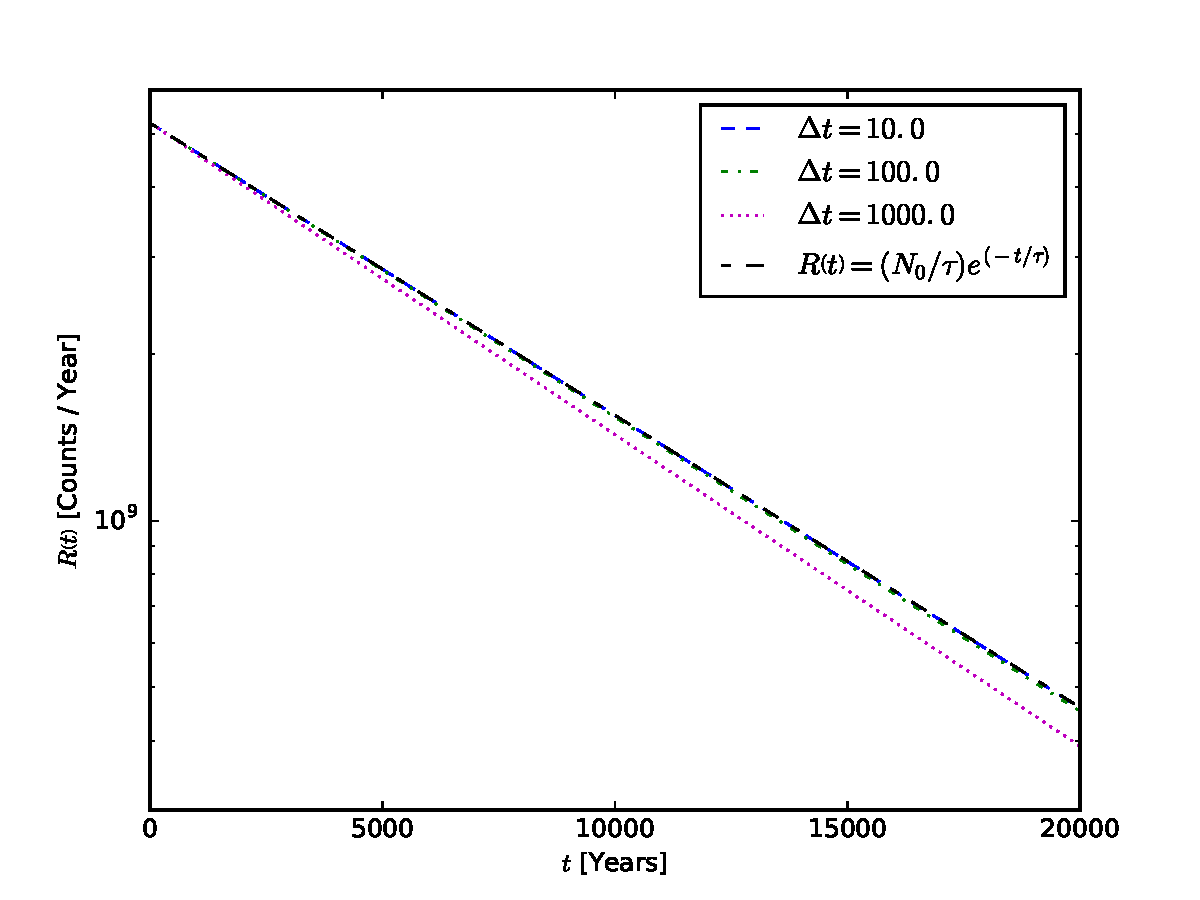
\includegraphics[width=.70\textwidth]{output/log_plot.pdf}
	{\par\nobreak\rule[9pt]{35em}{0.5pt}\vspace{-5mm}}
	\caption{Semi-log plot of $R\left(t\right)$ calculated numerically with three different time steps, $\Delta t$, and the exact solution.}
	\label{fig:log_plot}
\end{figure}

Besides just looking at plots, we can quantify how well the numerical results match the exact result by comparing them at specific times. A reasonable time to pick is $t = 2T_{1/2}$ (specified in the assignment itself) as the majority of nuclei have decayed by then, giving the numerical result sufficient time to diverge. Two useful variables for performing the comparison are the raw deviation, $R\left(t\right)_{exact}-R\left(t\right)_{numerical}$, and percent deviation, $100\%\cdot\left(R\left(t\right)_{exact}-R\left(t\right)_{numerical}\right)/R\left(t\right)_{exact}$. We can also compare the deviation to the second order term of the exact result, which can be found by expanding the exponential and identifying the correct term, $\left(N_{0}/\tau\right) \left(-t/\tau\right)^2/2$. The modeling code was modified to perform these calculations and print the results to the screen, see below: %Figure~\ref{lst:output}. % prints III instead of 1...
\newline
\lstinputlisting[style=output,label={lst:output}]{output/output.log}

As can be seen from the output, the percent deviation for both $\Delta t =$ 10 and 100 years is acceptable at \le 1\%. However setting $\Delta t =$ 1000 years results in a percent deviation of 9.2\% which is unacceptable for most applications. In this case using $\Delta t =$ 10 years is not computationally prohibitive, so there is no problem producing a high quality numerical result. Interestingly, it appears that the percent deviation and $\Delta t$ are linearly related, each increasing by an order of magnitude between the three different $\Delta t$'s. Of course this is only considering three data points and thus is a very weak observation, but it would be an interesting area for future investigation.

Upon taking the ratio of the deviations to the second order term of the exact result, we see that the deviations are orders of magnitude smaller than the second order term for all three time steps. This implies that only going to first order with Euler method was sufficient to model the decays behavior over the range of parameters considered, something hinted at immediately by how well the plots matched visually.

\section{Conclusions}
\label{sec:Conclusions}
The nuclear decay of Carbon-14, which must be well understood to facilitate the experimental method of Carbon dating, was successfully modeled numerically via the Euler method, as well as being solved analytically in Section~\ref{sec:theory}. Of the three time steps used, the shortest two produced acceptable results within \le1\% of the exact result while the longest was unacceptable with a 9.2\% deviation from the exact result. In all three cases the deviation from the exact result was much smaller in magnitude than the second order term of the analytic solution.

The Python source code used to produce these results can be found online at \url{http://github.com/mepland/PHYS_566_Computational_HW/tree/master/hw2/code}, and is included in Section~\ref{sec:code}.

\clearpage
\section{Supporting Material}
\label{sec:Supporting_Material}

\begin{figure}[!htbc]
%\begin{figure}
  \centering
  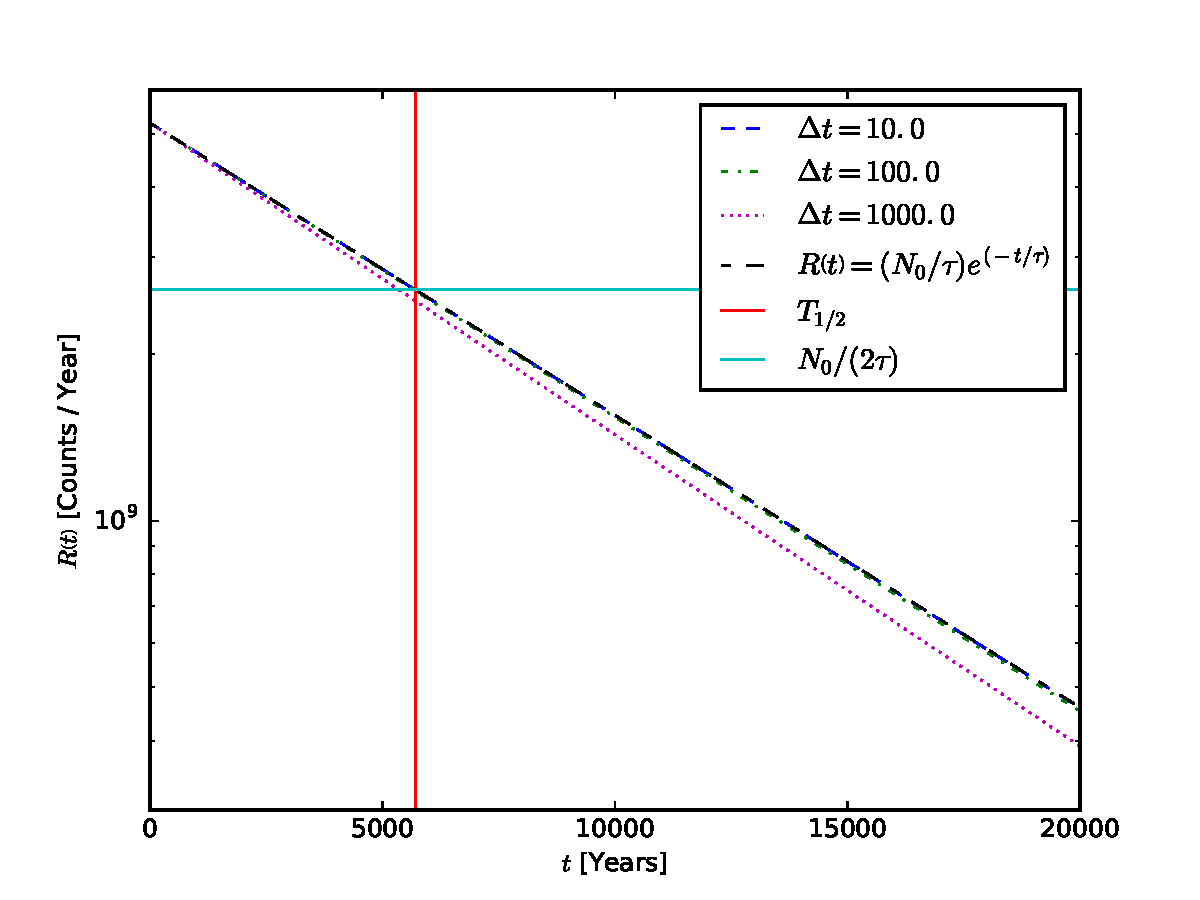
\includegraphics[width=.70\textwidth]{output/diagnostic_plot.pdf}
	{\par\nobreak\rule[9pt]{35em}{0.5pt}\vspace{-5mm}}
	\caption{$R\left(t\right)$ diagnostics plot generated to verify that $R\left(T_{1/2}\right) = \frac{N_{0}}{2\tau}$ as it should.}
	\label{fig:diagnostic_plot}
\end{figure}

\clearpage
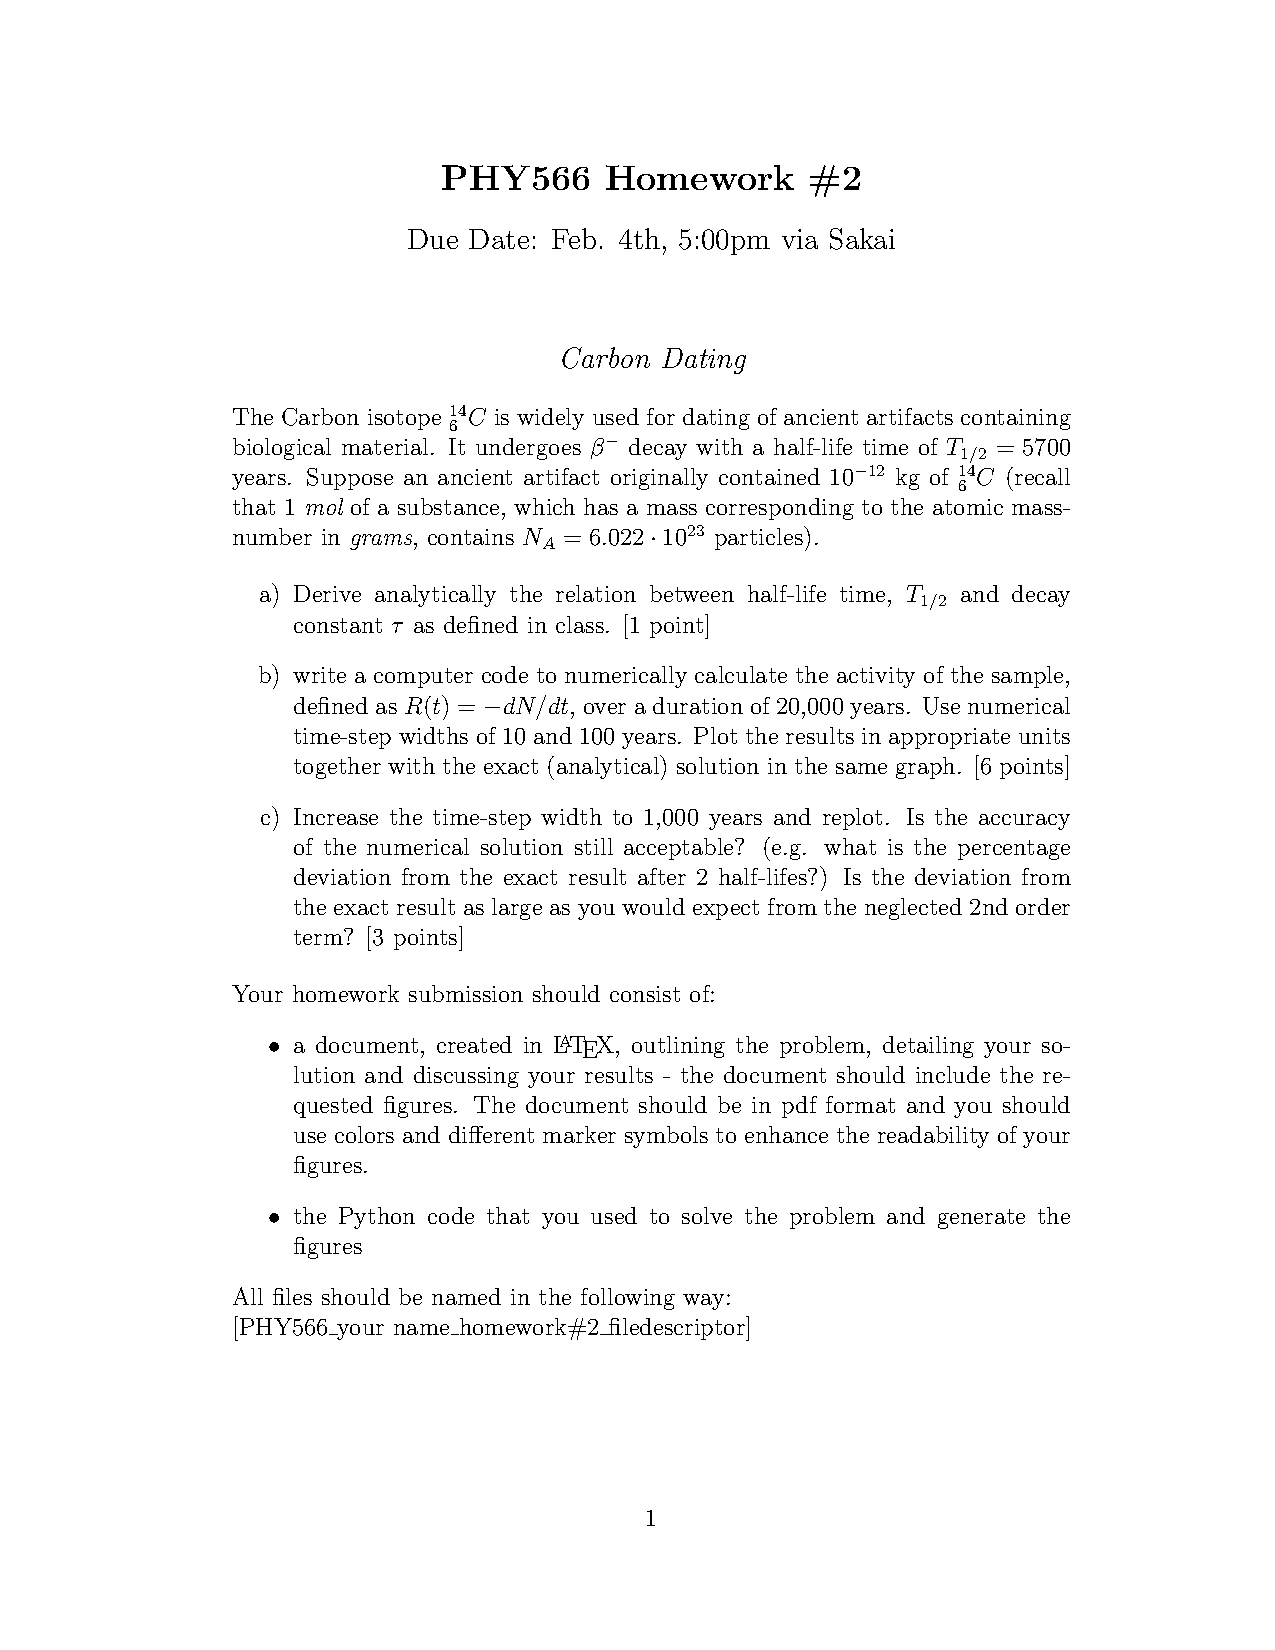
\includepdf{../homework2.pdf}

\clearpage
\section{Code}
\label{sec:code}

\lstinputlisting[style=python]{../code/exp_decay.py}

\end{document} %%% end of doc %%%




\bibliographystyle{bib_files/styles/atlasBibStyleWoTitle}
\bibliography{bib_files/my_bib.bib}


